\begin{comment}
\begin{itemize}
	\item The creatioon of Lender-Criteria bipartite graphs
	\item Explain why we could not project Lender-Criteria graphs onto Lender to create Lender-Lender graph
	\item That's why we find community directly in bipartite graphs
	\item Methodology: better-than-random testing
\end{itemize}

\section{Hypothesis testing on synthesis data}

\begin{itemize}
	\item How to build a random graph, with community pre-defined
	\item Detecting community in random graph
	\item Quality assessment of the detected community, presented by a numer $Q_{synthesis}$
	\item $Q_{synthesis}$ gives an idea about the best we could get from a data, but depends on the laten parameters when building datasets $p_{in}$, $p_{out}$, $p_{change}$ - the change from community to another
\end{itemize}

\section{Hypothesis testing on real data}

\begin{itemize}
	\item Filter data to keep Lenderes who is active invest from 2019-2023
	\item Repeat the works on random graph for each year data
	\item Then find quality assessment $Q_{real}$ again and compare with $Q_{synthesis}$.
	      Decide if there is a clear community for different criteria (Tags, Sectors, Country)
\end{itemize}
\end{comment}

As the begin of this chapter, we are revisiting our hypothesis and testing them out.
Recall that we would like to find community of Lenders, based on their interests in different criteria.
Through the data explornation, we will use 3 different criteria to find if the community exists.
The criteria are: Tags, Sectors and Country.

The first steps is to associate each Lender with Criteria.
In the Kiva data, Lender and Criteria are connected through the Project.
A Lender is considered to be interested in a Criteria if he/she has invested in a Project that has that Criteria.
Note that the relationship between Lender and Project is many-to-many.
The relationship between Project and Criteria could be many-to-many in the case of Tags,
or can be one-to-many in the case of Sectors and Country.
Because of the many-to-many relationship, we will model the data in Graph data type.
This decision is also supported by the fact that the "community finding" is a graph problem.
And by modeling the data in Graph, we can apply the work to other crowdfunding platforms.

\section{Lender-Criteria bipartite graph}

Like mention above we will use three Criteria features: Tags, Sectors and Country.
But in fact, Lenders do not have any direct relationships with Tags, Sectors or Country.
The relationship between Lender and Criteria is through the Project.
We consider that a Lender choose to invest in a Project because he/she is interested in the Criteria of that Project.
The interests could be explicitly, when a Lender actively find a project with sepecifics crietria.
For example, a Lender who intend to give money to Vietnamese people can search for
all the Projects that have the the Country criteria set to Vietnam.
That feature is available on Kiva website like described in previous chapter.
The interests could also be implicitly, which means that the Lender does not actively search for a Project with specific criteria.
For example, a Lender can contribute to a Project that he or she found on the homepage of Kiva,
and that Project has the Tag "Schooling".
He/she does not actively search for Projects with Tag "Schooling",
yet he/she contributes money to the projects.
We consider that the Lender is interested in the Tag "Schooling".


\begin{figure}[H]
	\centering
	\begin{subfigure}[b]{0.4\textwidth}
		\centering
		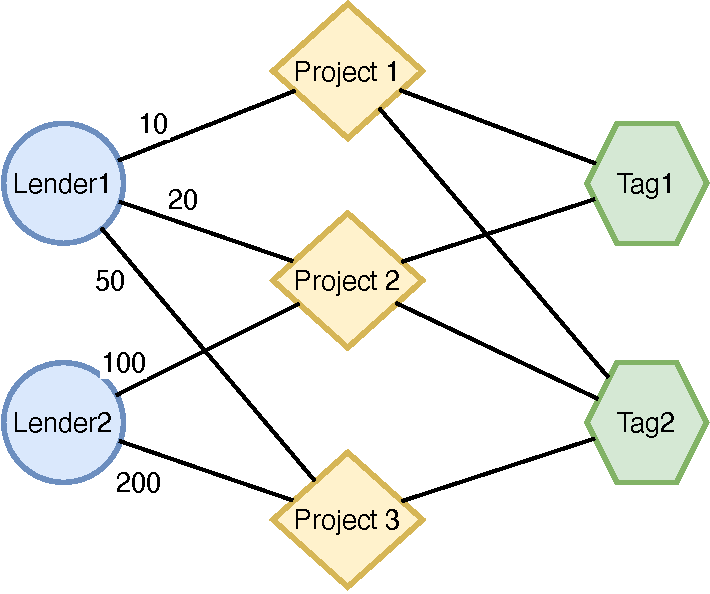
\includegraphics[width=0.8\textwidth]{images/schema_lender_tag.pdf}
		\caption{The relationship between Lender and Tag}
		\label{fig:schema_lender_tag}
	\end{subfigure}
	% \hfill
	\hspace{5mm}
	\begin{subfigure}[b]{0.4\textwidth}
		\centering
		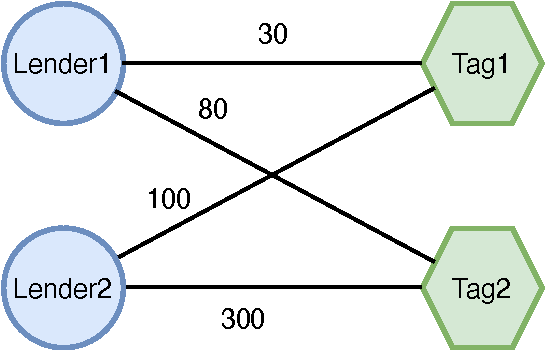
\includegraphics[width=0.6\textwidth]{images/create_lender_tag.pdf}
		\caption{The created Lender-Tag bipartite graph}
		\label{fig:create_lender_tag2}
	\end{subfigure}
	\caption{Process of creating the relationship between Lenders and Tags}
	\label{fig:create_lender_tag}
\end{figure}


Figure \ref{fig:create_lender_tag} illustrate the process of creating the relationship between Lenders and Tags.
For example, Lender1 has invested \$10 to Project1, \$20 to Project2 and \$50 to Project3.
Lender2 contributed \$100 to Project2 and \$200 to Project3.
Project1 was tagged with Tag1 and Tag2, the same for Project2, while Tag3 is the soly Tag of Project3.
We could see that Lender1 express his/her interest in Tag1 through two projects: Project1 and Project2.
We could further "weight" this interest by the amount of money that Lender1 contributed to Projects.
Lender1 contributed \$10 to Project1 and \$20 to Project2,
so we could say that Lender1 interest \$30 in Tag1.
By this way, we could construct a bipartite graph between Lenders and Tags like in Figure \ref{fig:create_lender_tag2}.

We also take this apportunity to mathematically define the notation that we will use in this chapter.
To list all the partites appear in our work, it would be Lender, Project, Tag, Sector and Country.
We will use the full name of the partite to denote the set of nodes in that partite.
For example, $Lender$ is the set of all Lenders.
For each member of each partite, we will use the first letter of the partite to denote the node.
For example, $L_1$ is a node in the set $Lender$.

Denote the graph in figure \ref{fig:schema_lender_tag}
\begin{equation}
	LPT(Lender, Project, Tag, LEND, TAGW)
\end{equation}

Where

\begin{itemize}
	\item $Lender \triangleq \{L_1, L_2, \ldots, L_i,\ldots \}$ is the set of Lenders. $0 \le i \le |Lender|$
	\item $Project \triangleq \{P_1, P_2, \ldots, P_j,\ldots \}$ is the set of Projects. $0 \le j \le |Project|$
	\item $Tag \triangleq \{T_1, T_2, \ldots, T_k,\ldots \}$ is the set of Tags. $0\le k \le |Tag|$
	\item $TAGW_{j,k}$ is the edges between Project $P_j$ and Tag $T_k$. $TAGW_{j,k} \in \{0, 1\}$
	\item $LEND_{i,j}$ is the edges between Lender $L_i$ and Project $P_j$,
	      It also is the amount of money in US dollar that $L_i$ contributed to $P_j$.
\end{itemize}

Note that the above is a 3-partite graph, which can be view as 2 bipartite graphs.
The first one is between Lenders and Projects

\begin{equation}
	LP(Lender, Project, LEND)
\end{equation}

The second one is between Projects and Tags

\begin{equation}
	PT(Project, Tag, TAGW)
\end{equation}

Denote the graph between Lenders and Tags as

\begin{equation}
	LT(Lender, Tag, INTEREST)
\end{equation}

Where the edge $INTEREST$ between Lender $L_i$ and Tag $T_k$ is the sum of amount of money that $L_i$ contributed to all Projects that have Tag $T_k$.

\begin{equation}
	INTEREST_{i,k}= \sum_{0\le j \le |Project|} LEND_{ij}\times TAGW_{jk}
\end{equation}

Follow the same logic, we could cosntruct the relationship between Lenders and Sectors, and between Lenders and Country.


\todo{add lines for raw dataset?}

\begin{table}[H]
	\centering
	\resizebox{\textwidth}{!}{%
		\begin{tabular}{|l|r|r|r|r|r|r|r|}
			\hline
			dataset        & $n_1$     & $n_2$     & $m$        & $k_1$ & $k_2$     & $k$   & $\delta$ \\
			\hline
			actor-movies   & 127,823   & 383,640   & 1,470,418  & 11.5  & 3.8       & 5.7   &
			0.000030                                                                                   \\
			authoring      & 19,885    & 16,400    & 45,904     & 2.3   & 2.8       & 2.5   & 0.00014  \\
			occurrences    & 13,587    & 9,264     & 183,363    & 13.5  & 19.8      & 16.0  & 0.0015   \\
			peer-to-peer   & 1,986,588 & 5,380,546 & 55,829,392 & 28.1  & 10.4      & 15.2  &
			0.0000052                                                                                  \\
			kiva LS        & 750793    & 15        & 3047733    & 4.06  & 203182.20 & 4.06  & 0.27     \\
			kiva LC        & 750793    & 93        & 5773899    & 7.69  & 62084.94  & 7.69  & 0.08     \\
			kiva LT        & 750793    & 60        & 7957291    & 10.60 & 132621.52 & 10.60 & 0.18     \\
			kiva active LS & 95662     & 15        & 659682     & 6.90  & 43978.80  & 6.89  & 0.46     \\
			kiva active LC & 95662     & 73        & 1453934    & 15.20 & 19916.90  & 15.19 & 0.21     \\
			kiva active LT & 95662     & 53        & 1640037    & 17.14 & 30944.09  & 17.13 & 0.32     \\
			\hline
		\end{tabular}%
	}
	\caption{Basic statistics of some bipartite graph datasets}
	\label{tab:bipartites-statistics}
\end{table}

Table \ref{tab:bipartites-statistics} shows the basic statistics of some bipartite graphs.
The first 4 graphs are from \cite{latapy2006}.
The last 6 graphs are from Kiva dataset.
Recall $n_1$ is the number of nodes in the first partite, $n_2$ is that for the second partite.
In the case of Kiva dataset, we set the first partite to be Lendre, and the second partite to be Tag, Sector or Country.
$m$ is the number of edges in the graph.
$k_1$ and $k_2$ are the average degree of nodes in the first and second partite respectively.
$k$ is the average degree of nodes in the graph.
$\delta$ is the density of the graph.
Notice that the kiva dataset is much denser than the other datasets,
and the average degree of nodes in the second partite is very high.

These number indicate the complexity of the kiva dataset.
Like mentioned in chapter 2, one of the way to study the community in bipartite graph is through one-mode projection.
Recall that when creating the one-mode projection (onto Lender for instance),
each nodes in the other mode (i.e. a Tag) will generate $\frac{d(d-1)}{2}$ iterations,
where $d$ is the degree of that (Tag) node.
Take the kiva active LS dataset for example.
It has the average Sector degree is $k_2=43978.80 \approx 4.4\times 10^4$.
The required iterations for create the one-mode projection is
$4.4\times 10^4 \times (4.4\times 10^4 - 1) \approx 1.93 \times 10^9$.
This is a huge number, and it is infeasible to create the one-mode projection, let alone to analyze it.

But we have to take a moment to express that this resonale is not obvious for us at the beginning.
Having the kiva dataset in hand, we have naively try to create the one-mode projection for studying the community in it.
The initial perception was that the task was too slow, might be because of the tools that we use.
At first, it seems that using only python and pandas is too slow for the task.
So we spend time try it with various tools, from the popular database PostgresSQL,
to the type of database that is specifically designed for handle graph-like data: Neo4j and Memgraph.
We even manage to try GPU-accelerated tools like cuDF and cuGraph,
taking to a next level by using distributed computing with Dask.
Only since all of these tools are not enough to handle the projection,
we realize that we have missed something.
Then we come back to literature and find out that it is impossible to create the projection with our dataset.
We decided to use the bipartite graph directly for community detection.
In chap2, we have mentioned that most works on this topic are supervised tasks,
meaning that the community is known beforehand.
While in our case, we do not know the community, and we have to find it out.
Hence in order to assess the quality of the community that we found,
we adopt the better-than-random methodology well-known in the literature.


% \todo{degree distribution \cite{latapy2006}}

\todo{Transaction to next chapter}

\section{Hypothesis testing on synthesis data}

In this section, we will build a dynamic bipartite graph with predefined community.
We will use this graph to test a community detection algorithm.
The community detection algorithm will be applied to the real data in the next section.

We will create a bipartite graph with 2 partites: $V_1$ and $V_2$.
The number of nodes in each partite is $n_1$ and $n_2$ respectively.
We choose the to fix $n_1$ and $n_2$ to be the same as the kiva dataset,
hence $n_1=7000, n_2=25$.

Then we define the communtiy structure of the graph.
We predefined that in each partite, there are $n_{community} = 5$ communities.
Look at the figure \ref{fig:synthesis_graph} for illustration.
Two partites represented by two type of nodes: Circle and Diamond.
At the first time $T_1$, the community structure is predefined, showing by the rounded rectangles, they are $C_1, C_2, D_1, D_2$.
We also intend to make the co-cluster beforehand.
That is $C_1$ and $D_1$ are intended to be co-cluster, $C_2$ should be co-cluster mate of $D_2$.
Note that $n_{community} = 5$ means we have 5 co-cluster pairs.
In order to generate this structure, we employ two parameters $p_{in}$ and $p_{out}$.
$p_{in}$ is the probability that a node in $V_1$ is connected to a node in $V_2$ if they are in the same co-cluster.
A node in $V_1$ could connect to a different co-cluster node in $V_2$ with probability $p_{out}$.
We have to set $p_{in} > p_{out}$ to make sure that the co-cluster pairs are more connected than the other pairs.

In fact, we will generate the graph dynamically.
There are several snapshot of the data at different time $T_1, T_2, \ldots, T_T$.
The above generation process is applied for the first snapshot only.
For next snapshots, community structure could be change with with a new variable $p_{stay}$.
We mimic the behavior of a Lender here, that is a node in $V_1$ could change its community over time.
$p_{stay1}$ is the probability that a node in $V_1$ stay in the same community from time $T_i$ to $T_{i+1}$,
and it can switch to a new community with probability $1-p_{stay1}$ as illustrated in figure \ref{fig:synthesis_graph}.
The same goes for $V_2$ with $p_{stay2}$.
The cocluster relationship will be predefined and kept the same over time.
The details of the algorithm is described in \ref{alg:synthesis_graph_all}.

Now we already have multiple bipartite graphs for each timestamp.
We also have the community structure - the ground truth for each timestamp.
We will apply the community detection algorithm to each bipartite graph,
and compare the result with the ground truth.
We defined a metric $Q$ based on Jaccard Index, to measure the quality of the community detection result.
Consider the $k$ ground-truth clusters $\{U_1, \ldots, U_k\}$
and let $\{\tilde{U}_1, \ldots, \tilde{U}_s\}$ be the $s$ clusters returned by an algorithm.
The quality $Q$ of the solution $\tilde{U}_j$ is computed as follows.
For each ground-truth cluster $U_i$, find the cluster $\tilde{U}_j$
which maximizes the Jaccard coefficient of $U_i$ and $\tilde{U}_j$.
Then sum over the Jaccard coefficients for all ground-truth clusters $U_i$ and normalize by $k$.
Formally,

\begin{equation}
	Q=\frac{1}{k} \sum_{i=1}^k \max _{j=1, \ldots, s} J\left(U_i, \tilde{U}_j\right)
\end{equation}

where $J(A, B)=|A \cap B| /|A \cup B|$ is the Jaccard coefficient.
$Q \in [0,1]$, higher values for $Q$ imply a better quality of the solution.
E.g., if $Q=1$ then the clusters $\tilde{U}_j$ match exactly the ground-truth clusters $U_i$.


\begin{algorithm}[H]
	\caption{Synthesis graph generation}
	\label{alg:synthesis_graph_all}
	\begin{description}
		\item[Input:] $T$ \Comment{Number of timestep}
		\item[Input:] $n_1, n_2$ \Comment{Number of nodes for each partite}
		\item[Input:] $c_1, c_2$ \Comment{Number of community for each partite}
		\item[Input:] $p_{stay1}, p_{stay2}$ \Comment{Probability of staying in the same community}
		\item[Input:] $p_{in}$ \Comment{Probability of connecting to a node in the same community}
		\item[Input:] $p_{out}$ \Comment{Probability of connecting to a node in a different community}
		\item[Output:] biajacency matrixes $B \in \mathbb{R}^{T \times n_1 \times n_2}$
		\item[Output:] community indexes $C \in \mathbb{N}^{T \times n_1}$
		\item[Output:] community indexes $D \in \mathbb{N}^{T \times n_2}$
	\end{description}
	\begin{algorithmic}[1]
		\State $B \gets$ \Call{zeros}{$T, n_1, n_2$}
		\State $C \gets$ \Call{generate\_community\_dynamic\ref{alg:appendix-synthesis_graph_nodes}}{$T$, $n_1$, $c_1, p_{stay1}$}
		\State $D \gets$ \Call{generate\_community\_dynamic\ref{alg:appendix-synthesis_graph_nodes}}{$T$, $n_2$, $c_2, p_{stay2}$}
		\State $M \gets$ \Call{generate\_cocluster\ref{alg:appendix-synthesis_graph_cocluster}}{$c_1, c_2$}
		\Comment cocluster stay the same over time
		\For {$t=1,2,\ldots,T$}
		\State \Call {generate\_edges\ref{alg:appendix-synthesis_graph_edges}}{$B[t], C[t], D[t], p_{in}, p_{out}$}
		\EndFor
	\end{algorithmic}
\end{algorithm}



\begin{figure}[H]
	\centering
	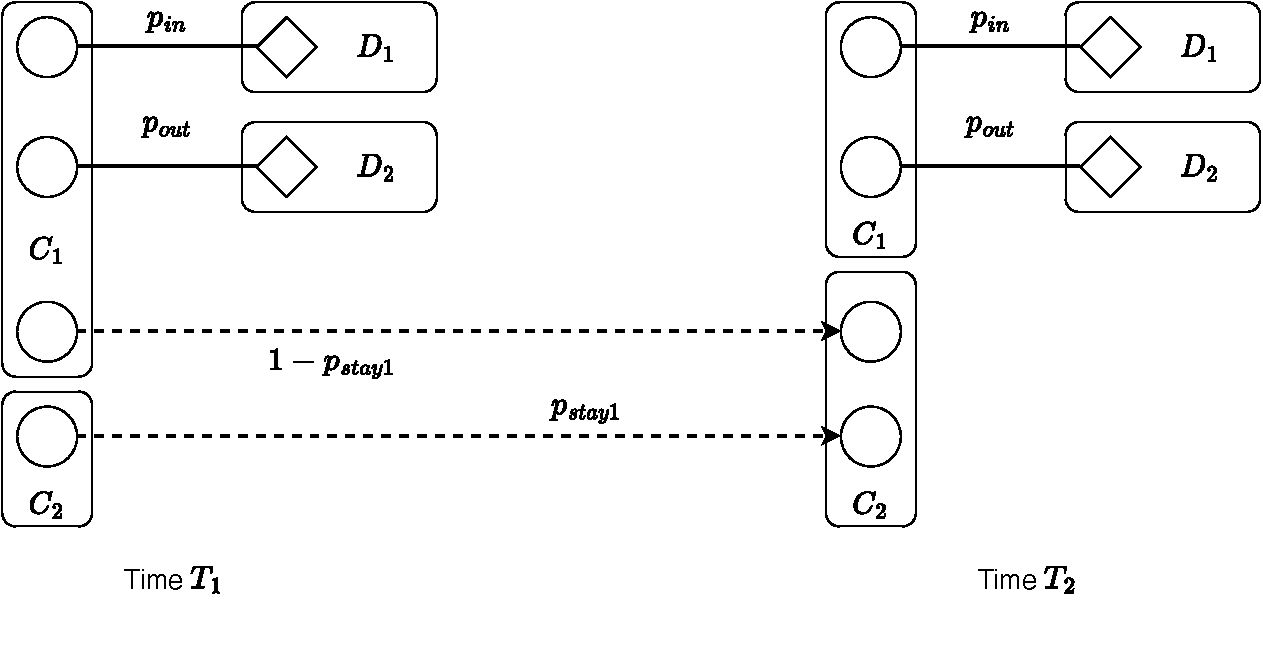
\includegraphics[width=0.8\textwidth]{images/synthesis.pdf}
	\caption{Illustrate the process of creating the synthesis bipartite graph.}
	\label{fig:synthesis_graph}
\end{figure}

\todo{describe the algorithm. then provide our init condition $p_{stay1} = p_{stay2}$ for example}

We will conduct an experiment to test what is the $Q$ value for different parameters.
Choose the parameters $n_1 = 7000, n_2 = 25, n_{community} = 5, T=5$.
We fix the value $p_{in} = 0.95, p_{stay2}$, while vary the value of $p_{stay1}$ in range $[0, 1]$ and $p_{out}$ in range $[0, 0.5]$.
Notice that $p_{out} < p_{in}$, otherwise the community structure is not meaningful.
With each parameters setting, we will generate 20 different graphs with different random seed.
Then we will apply the community detection algorithm to each graph and compute the $Q1$ value,
which is the $Q$ value for the $V_1$ partite.

We employ the biLouvian algorithm as mentioned in Chapter 2 for detecting the community.
Note that the algorithm use Murata+ to metric to tell how good the finding is.
Figure \ref{fig:modularity_pout} shows that metric as a function of $p_{out}$.
We could see that \todo{here}
We could see that the $modularity$ is tend to be high when $p_{out}$ is low.
Recall that we set $p_{in}$ fixed at $0.95$.
When $p_{out}$ is low, the difference between edge density in pre-defined community and the other is high.
The algorithm works well on this case.
For an extreme case when $p_{out} = 0$, the graph has no edge between different community.
The community structure is very clear, hence the algorithm suppose to work well.
In fact, the algorithm yield the bimodularity close to $1.0$ in this case.
When $p_{out} = 0.05$, there still be a clear structure because the probability
of connecting to a node in a different community is $~20$ times lower than
connecting to a node in a same community.
In this case, the algorithm still works well, it produce the bimodularity fluctuate around $0.6$.
The higher $p_{out}$ is, the more difficult for the algorithm to find the community.
But when $p_{out} \ge 0.2$, the metric seem to be set still at $0.5$.
We look at the results and found that the algorithm detected the whole graph as a single cocluster.

\begin{figure}[H]
	\centering
	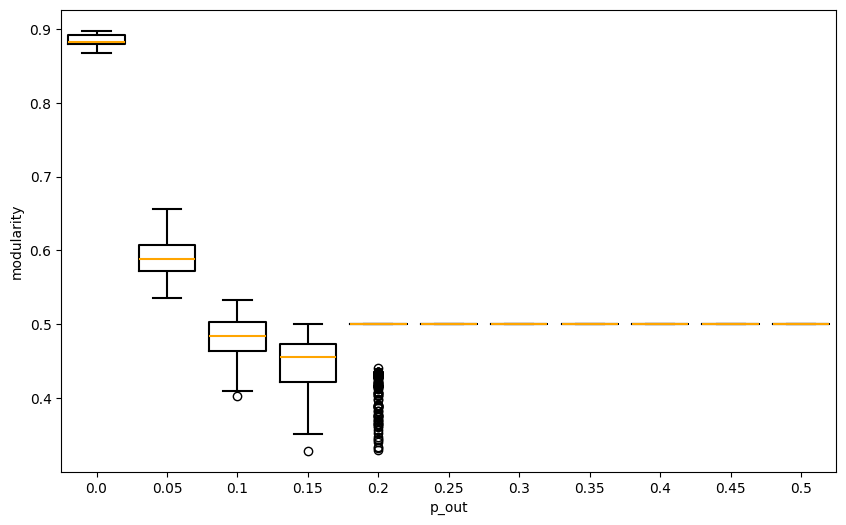
\includegraphics[width=0.8\textwidth]{images/modularity_pout.png}
	\caption{$modularity$ as a function of $p_{out}$ }
	\label{fig:modularity_pout}
\end{figure}

Moving next to the $Q1$ value, recall that $Q1$ measure the similarity between detected community in $V_1$ and the ground truth.
Figure \ref{fig:Q1_pout} shows that $Q1$ is tend to be high when $p_{out}$ is low.
The algorithm works as expected in the extreme case when $p_{out} = 0$.
When $p_{out} = 0.05$ and $p_{out} = 0.1$, the algorithm still works well, it produce the $Q1$ fluctuate around $0.65$ and $0.5$ respectively.
The behavior in $Q1$ is consistnent with the $modularity$ metric.
When $p_{out} \ge 0.2$, the algorithm detected the whole graph as a single cocluster.
And because we preset the number of community in $V_1$ to be $c_1=5$,
Hence when the whole graph is detected as a single cocluster, the $Q1$ value is $0.2$.

\begin{figure}[H]
	\centering
	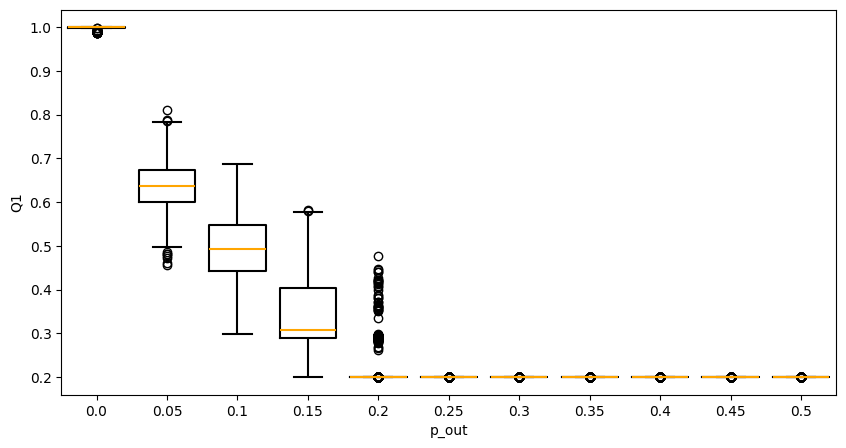
\includegraphics[width=0.8\textwidth]{images/Q1_pout.png}
	\caption{$Q1$ as a function of $p_{out}$ }
	\label{fig:Q1_pout}
\end{figure}

The results reveal that the algorithm only works well when the difference between edge density in pre-defined community and the other is high.
We could get a sense of the value range of $Q1$.
For example, even the difference is quite large when $p_{out}=0.15$,
$Q1$ only archieve around $0.3$, meaning that the algorithm only detect $30\%$ of the community.
It indicate that in the real dataset, if we manage to find a community that
its member remain roughly $30\%$ over time, we can be confident that the community is real.

\todo{refine the $p_{stay2}$}


\section{Hypothesis testing on real data}

\begin{itemize}
	\item
	\item Filter data to keep Lenderes who is active invest from 2019-2023
	\item Repeat the works on random graph for each year data
	\item Then find quality assessment $Q_{real}$ again and compare with $Q_{synthesis}$.
	      Decide if there is a clear community for different criteria (Tags, Sectors, Country)
\end{itemize}

% \include{images/tikz/LCountry.tex}

The results is not easy to visualize but we will try our best to explain it here.
Figure \ref{fig:appendix-LSector} shows the result of Lender-Sector community detection.
The results looks like a graph where each node represents a co-cluster.
We could not list all the member of a cocluster because there are too many of them,
but only show some Sectors in each cocluster.
Edges represents the similarities between co-clusters, which recall that is the Jaccard Index.
Each label of a edge is a tuple of similarity of Lender nodes and Sector nodes.
We try to align the result with timeline from 2019 to 2023 as shown.
The thickness of the edge is proportional to the maximum similarity $max(\text{lender\_similarity}, \text{sector\_similarity})$.
In this way, one should focus on edges with high thickness.

\begin{figure}[H]
	\centering
	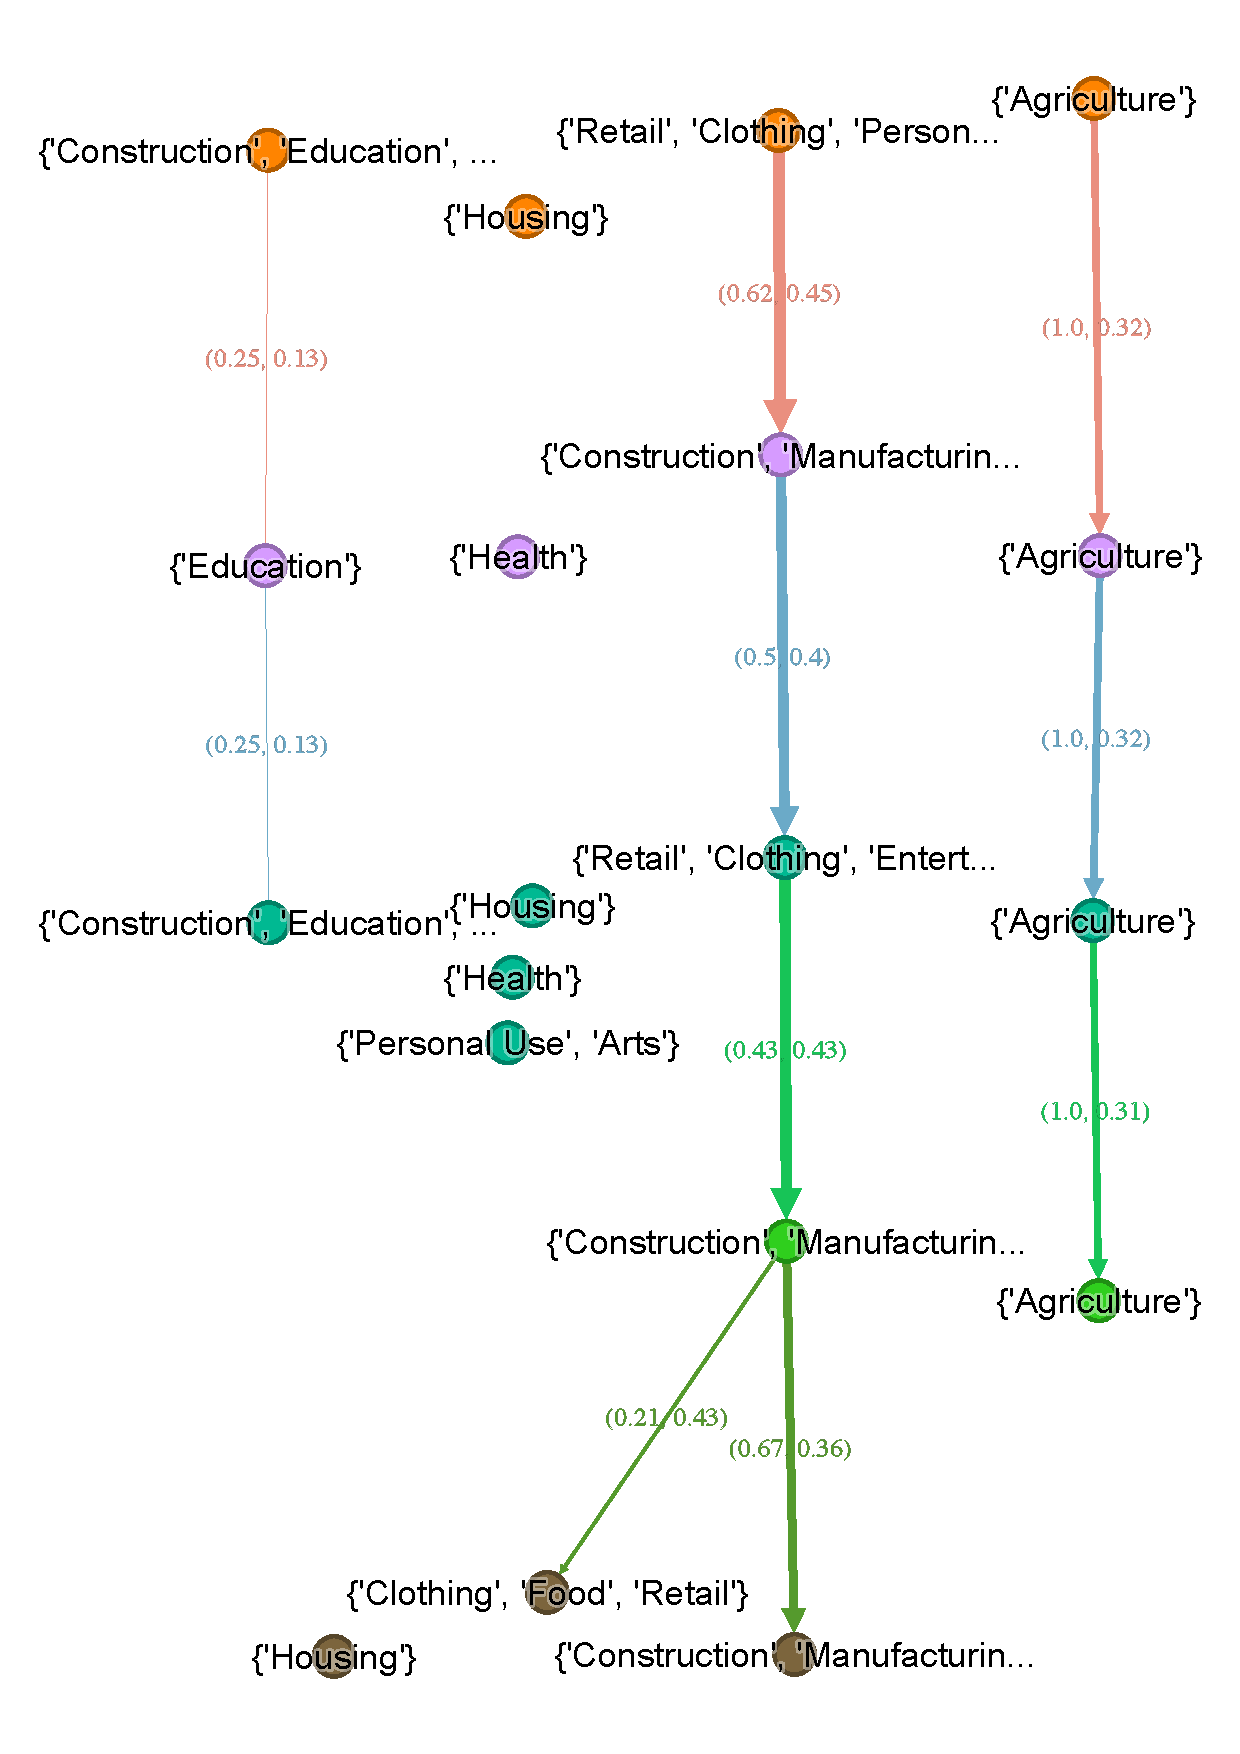
\includegraphics[width=0.8\textwidth]{images/LSector.pdf}
	\caption{Illustrate the result of Lender-Sector community detection.}
	\label{fig:appendix-LSector}
\end{figure}

Look at the figure, we could identify some interesting patterns.
Take the part of the graph in the red rectangle for example.
We could see a clear line structure here.
Each nodes in this line represent a cocluster in a year,
notice that all these cocluster are in the same Sector: Agriculture.
Table \ref{tab:LS-agriculture} shows the details of the cocluster in Agriculture Sector.

\todo{where the users go??????????}


\begin{table}[H]
	\centering
	\resizebox{\textwidth}{!}{%
		\begin{tabular}{lllrr}
			\hline
			time       & community\_lender                                                             & community\_tag  & lender\_similarity\_to\_lastyear & tag\_similarity\_to\_last\_year \\
			\hline
			2019-01-01 & ['helen6472', 'becki2967', 'steohen6319', 'broen4509', 'mark6805', '...']     & {'Agriculture'} & -                                & -                               \\
			2020-01-01 & ['helen6472', 'steohen6319', 'broen4509', 'mark6805', 'kelsey6209', '...']    & {'Agriculture'} & 0.318373                         & 1.000000                        \\
			2021-01-01 & ['becki2967', 'steohen6319', 'fabianfuchs', 'tracy4274', 'mark6805', '...']   & {'Agriculture'} & 0.323045                         & 1.000000                        \\
			2022-01-01 & ['becki2967', 'holly4656', 'kelsey6209', 'patricia4011', 'gerben5289', '...'] & {'Agriculture'} & 0.313389                         & 1.000000                        \\
			\hline
		\end{tabular}
	}
	\caption{A result in Lender-Sector community detection}
	\label{tab:LS-agriculture}
\end{table}

